\documentclass[a4paper,12pt]{article}
\usepackage{setspace}\setstretch{1.5}
\usepackage[T1]{fontenc}
\usepackage[utf8]{inputenc}
\usepackage{graphicx}
\usepackage{subcaption}
%\usepackage[Conny]{fncychap}
\usepackage{amsmath,amssymb}
\usepackage{fullpage}
\usepackage{ragged2e}
\usepackage{rotating}
\usepackage{multicol}
\usepackage{tabularx}
\usepackage{float}
\usepackage{titlesec}
\usepackage{titling}
%\numberwithin{figure}{section}
\usepackage{adjustbox}
\usepackage{parskip}
\usepackage{listings}
\usepackage{xcolor}
\usepackage[final]{pdfpages}
\usepackage[toc,page]{appendix}
\usepackage[margin=0.75in]{geometry}
\usepackage{gensymb}
\usepackage{tgbonum}	      % a font package
\usepackage{booktabs}       % making tables prettier
\renewcommand{\arraystretch}{1.3}


%\color{violet}

\renewcommand{\familydefault}{\sfdefault}

\captionsetup{font=footnotesize, labelfont={bf,sf}}

\raggedbottom

%\def\ga2o3{Ga$_2$O$_3$}
\def\ga2o3{$\beta$-Ga$_2$O$_3$}
\def\cheq{\leftrightharpoons}
\def\deg{$^\circ$C$_{}$}
\date{}
\author{Vilde Mari Reinertsen}

\title{\LARGE {\fontfamily{phv}\selectfont A graduate student's quest to find out: \\Is my research scientific?\\ \vspace{0.7cm} \large A comparison of my methods with different proposed scientific methods} \\}

\begin{document}
\begingroup
\let\center\flushleft
\let\endcenter\endflushleft
\maketitle
\endgroup

\section{The derivatives and the local energy}

In order to find the drift force and the local energy analytically we need to calculate both the derivative and the double derivative of the trial wavefunction.

\subsection{The derivative of the trial wave function}

We separate the total trial wave function (Eq. \ref{eq:trialwf}) into the one-body part and the interaction part,
\begin{equation}
\Psi_T = \Psi_{ob}\Psi_{in}.
\end{equation}

Using the product rule, the derivative with regards to the particle $k$ is
$$ \nabla_k \Psi_T =  \Psi_{ob}\nabla_k\Psi_{in} + \nabla_k\Psi_{ob}\Psi_{in}.$$
(Here the operator $\nabla_k$ only works on the first function after it.)

So we have to calculate $\nabla_k\Psi_{ob}$ and $\nabla_k\Psi_{in}$ and insert the expressions into the equation above.

We have (if $g(\mathbf{r}_k,\alpha) = \phi(\mathbf{r}_k)$)
\begin{equation}\label{eq:psi_ob_derivative}
\nabla_k\Psi_{ob} = \nabla_k \phi(\mathbf{r}_k)\prod_{k\neq i}^N \phi(\mathbf{r}_i)= \frac{\nabla_k \phi(\mathbf{r}_k)}{\phi(\mathbf{r}_k)} \Psi_{ob}
\end{equation}
using the chain rule.

The interaction part is a little more complicated. We start with
$$ \nabla_k\Psi_{in} = \nabla_k  \exp{\left(\sum_{j<i}u(r_{ji})\right)} = \exp{\left(\sum_{j<i}u(r_{ji})\right)} \sum^N_{l \neq k}  u\left(r_{kl}\right) \nabla_k u (r_{kl}) $$. Because it is an exponential function we have to multiply the original function with the sum over all the terms in the exponent that are dependant on the particle $k$. Because $u(r_{kj}) = u(r_{jk})$ this sum is $\sum^N_{l \neq k}  u\left(r_{kl}\right)$. In addition we have to multiply with the derivative of $u(r_{kl})$ because of the chain rule. Since we have a sort of simplified way of showing the derivative (using the operator $\nabla_k$), the expression $u(r_{kj})\nabla_k u(r_{kj}) = \nabla_k u(r_{kj})$ by using the chain rule the opposite way. We then have the expression

\begin{equation}\label{eq:psi_in_derivative}
\nabla_k\Psi_{in} = \exp{\left(\sum_{j<i}u(r_{ji})\right)} \sum^N_{l \neq k} \nabla_k u (r_{kl}) = \sum^N_{l \neq k} \nabla_k u (r_{kl}) \Psi_{in}
\end{equation}
for the derivative of the interaction part of the wave function.

The total expression of the derivative of the trial wave function is hence 
\begin{align}
\nabla_k \Psi_T &= \Psi_{ob}\nabla_k\Psi_{in} + \nabla_k\Psi_{ob}\Psi_{in}\\
 &= \prod_{k\neq i}^N \phi(\mathbf{r}_i)\exp{\left(\sum_{j<i}u(r_{ji})\right)} \sum^N_{l \neq k} \nabla_k u (r_{kl}) + \nabla_k \phi(\mathbf{r}_k)\prod_{k\neq i}^N \phi(\mathbf{r}_i) \exp{\left(\sum_{j<i}u(r_{ji})\right)}\\
 &= \Psi_{ob}\sum^N_{l \neq k} \nabla_k u (r_{kl}) \Psi_{in}+ \frac{\nabla_k \phi(\mathbf{r}_k)}{\phi(\mathbf{r}_k)} \Psi_{ob}\Psi_{in}\\
 &= \left(\sum^N_{l \neq k} \nabla_k u (r_{kl})+ \frac{\nabla_k \phi(\mathbf{r}_k)}{\phi(\mathbf{r}_k)}\right) \Psi_T 
\end{align}

\subsection{The double derivative of the trial wave function}

The double derivative with regards to particle $k$ is

\begin{equation}\label{eq:total_double_start}
nabla^2_k \Psi_T =  \Psi_{ob}\nabla^2_k\Psi_{in} + 2\nabla_k\Psi_{ob}\nabla_k\Psi_{in} + \Psi_{ob}\nabla^2_k\Psi_{in}.
\end{equation}
So we have to calculate $\nabla^2_k\Psi_{ob}$ and $\nabla^2_k\Psi_{in}$, in addition to the derivatives form the previous section, and insert the expressions into the equation above.

From Eq. \ref{eq:psi_ob_derivative} we find
$$ \nabla^2_k\Psi_{ob} = \nabla^2_k \phi(\mathbf{r}_k)\prod_{k\neq i}^N \phi(\mathbf{r}_i) = \frac{\nabla^2_k \phi(\mathbf{r}_k)}{\phi(\mathbf{r}_k)} \Psi_{ob},$$
since $\prod_{k\neq i}^N \phi(\mathbf{r}_i)$ is independent of the particle $k$.

For the double derivative of $\Psi_{in}$ we use the product rule again
\begin{equation}\label{eq:double_derivative_start}
\nabla^2_k\Psi_{in} = \exp{\left(\sum_{j<i}u(r_{ji})\right)} \nabla_k\left[ \sum^N_{l \neq k} \nabla_k u (r_{kl})\right] +\nabla_k\left[ \exp{\left(\sum_{j<i}u(r_{ji})\right)}\right] \sum^N_{l \neq k} \nabla_k u (r_{kl}).
\end{equation}
Here the square brackets are used to show what $\nabla_k$ applies to. So,

$$\nabla_k\left[ \exp{\left(\sum_{j<i}u(r_{ji})\right)}\right]=  \exp{\left(\sum_{j<i}u(r_{ji})\right)} \sum^N_{l' \neq k} \nabla_k u (r_{kl'})$$ as in the previous section. We calculate $ \nabla_k u(r_{kl'})$ using the chain rule and get
$$ \nabla_k u(r_{kl'})  = \frac{\mathbf{r}_k - \mathbf{r}_{l'}}{r_{kl'}} u'(r_{kl'}), $$ where $u'(r_{kl'}) = \frac{d}{dr_{kl'}}u(r_{kl'})$, because $$\frac{d}{d\mathbf{r}_{k}}r_{kl'} =\frac{d}{d\mathbf{r}_k}\sqrt{(x_k-x_{l'})^2 + (y_k-y_{l'})^2 + (z_k-z_{l'})^2} = \frac{\mathbf{r}_k - \mathbf{r}_{l'}}{r_{kl'}} $$ and then
$$\nabla_k\left[ \exp{\left(\sum_{j<i}u(r_{ji})\right)}\right]=  \exp{\left(\sum_{j<i}u(r_{ji})\right)} \sum^N_{l' \neq k} \frac{\mathbf{r}_k - \mathbf{r}_{l'}}{r_{kl'}} u'(r_{kl'}) = \Psi_{in} \sum^N_{l' \neq k} \frac{\mathbf{r}_k - \mathbf{r}_{l'}}{r_{kl'}} u'(r_{kl'})  $$

Next, we have
\begin{equation}\label{eq:double_der_part_in}
\nabla_k\left[ \sum^N_{l \neq k} \nabla_k u (r_{kl})\right] = \nabla_k \left[ \sum^N_{l \neq k}  \Psi_{in} \frac{\mathbf{r}_k - \mathbf{r}_{l}}{r_{kl}} u'(r_{kl}) \right] = \sum^N_{l \neq k} \nabla_k \left[ d \cdot \frac{a}{b} \cdot c \right]
\end{equation}
where $a = \left(\mathbf{r}_k-\mathbf{r}_{l}\right)$, $b= r_{kl}=|\mathbf{r}_k-\mathbf{r}_{l}|$ , $c = u'(r_{kl})$ and $d = \Psi_{in}= \exp\left(\sum_{i<j}^N u(r_{ij})\right)$. Furthermore, $a' = \frac{d}{d\mathbf{r}_k} \left(\mathbf{r}_k-\mathbf{r}_{l}\right) = \frac{d}{dx_k} x_k  + \frac{d}{dy_k} y_k  +\frac{d}{dz_k} z_k   = 3$ (the number of dimensions), $b' = \frac{d}{d\mathbf{r}_k} r_{kl} = \frac{\mathbf{r}_k - \mathbf{r}_{l}}{r_{kl}}$, $c' = \frac{d}{d\mathbf{r}_k} u'(r_{kl}) =  u''(r_{kl})\frac{\mathbf{r}_k - \mathbf{r}_{l}}{r_{kl}}$ and $d' = \Psi_{in} \sum^N_{l \neq k} \frac{\mathbf{r}_k - \mathbf{r}_{l}}{r_{kl}} u'(r_{kl})$. Inserting all these expression into Eq. \ref{eq:double_der_part_in} gives (skipping some of the simplifications since the explanation is in the above part)
\begin{align}
\nabla_k\left[ \sum^N_{l \neq k} \nabla_k u (r_{kl})\right] &= \sum^N_{l \neq k} \left( \left(\frac{3r_{kl}}{\left(\mathbf{r}_k-\mathbf{r}_{l}\right)^2}-\frac{1}{r_{kl}}\right)u'(r_{kl}) + u''(r_{kl})\right) \frac{\left(\mathbf{r}_k-\mathbf{r}_{l}\right)^2}{r_{kl}^2} \Psi_{in} \\ \label{eq:doble_der_u}
&= \sum^N_{l \neq k} \left( \frac{2}{r_{kl}}u'(r_{kl}) + u''(r_{kl})\right) \Psi_{in}
\end{align}
When we insert the results into Eq. \ref{eq:double_derivative_start} we get
$$\nabla^2_k\Psi_{in} = \Psi_{in}\sum^N_{l \neq k} \left( \frac{2}{r_{kl}}u'(r_{kl}) + u''(r_{kl})\right) \Psi_{in} +  \Psi_{in} \sum^N_{l' \neq k} \frac{\mathbf{r}_k - \mathbf{r}_{l'}}{r_{kl'}} u'(r_{kl'}) \Psi_{in} \sum^N_{l \neq k} \frac{\mathbf{r}_k - \mathbf{r}_{l}}{r_{kl}} u'(r_{kl})  $$

$$\nabla^2_k\Psi_{in} = \Psi^2_{in} \left[\sum^N_{l \neq k} \left( \frac{2}{r_{kl}}u'(r_{kl}) + u''(r_{kl})\right) +   \sum^N_{l' \neq k} \sum^N_{l \neq k} \frac{(\mathbf{r}_k - \mathbf{r}_{l'})(\mathbf{r}_k - \mathbf{r}_{l})}{r_{kl'}r_{kl}}  u'(r_{kl})u'(r_{kl'}) \right] $$

Inserting it all into Eq. \ref{eq:double_derivative_start} and dividing by the trial wavefunction (as we will do to find the local energy) gives
\begin{align*}
   \frac{1}{\Psi_T(\mathbf{r})}\nabla_k^2\Psi_T(\mathbf{r})
   &= \frac{\nabla_k^2\phi(\mathbf{r}_k)}{\phi(\mathbf{r}_k)}
   + 2\frac{\nabla_k\phi(\mathbf{r}_k)}{\phi(\mathbf{r}_k)}
   \left(\sum_{l\ne k}\frac{(\mathbf{r}_k-\mathbf{r}_l)}{r_{kl}}u'(r_{kl})\right)
   \\
   &\qquad
   + \sum_{l\ne k}\sum_{l' \ne k}\frac{(\mathbf{r}_k-\mathbf{r}_l)(\mathbf{r}_k-\mathbf{r}_{l'})}{r_{kl}r_{kl'}}u'(r_{kl})u'(r_{kl'})
   \\
   &\qquad
   + \sum_{l\ne k}\left( u''(r_{kl})+\frac{2}{r_{kl}}u'(r_{kl})\right).
\end{align*}

\section{The local energy and drift force as implemented in the code}\label{sec:implementation}

To calculate the kinetic energy part of the local energy we use the last expression in the previous section, summed over all particles $k$. We use $\phi(\mathbf{r}_k)$ from Eq. \ref{eq:phi} and find 

$$ \sum_k^N\frac{\nabla_k^2\phi(\mathbf{r}_k)}{\phi(\mathbf{r}_k)} = -2\alpha Nd + 4 \alpha^2 \sum_k^N \mathbf{r}_k^2 $$ where $d$ is the number of dimensions and $\mathbf{r}_k^2 = x_k^2 + y_k^2+\beta z_k^2$. This is the expression for the kinetic part of the local energy if there is no interaction. Furthermore, from Eq. \ref{eq:phi} and Eq. \ref{eq:psi_ob_derivative}

$$ \frac{\nabla_k\phi(\mathbf{r}_k)}{\phi(\mathbf{r}_k)} = -2\alpha  \mathbf{r}_k $$
 
We also have
\begin{align*}
u'(r_{kl}) &= -\frac{a}{ar_{kl}-r_{kl}^2} \text{ and }\\
u''(r_{kl}) ) &= \frac{a(a-2r_{kl})}{r_{kl}^2(a-r_{kl})^2}
\end{align*} for $r_{kl} > a$. The other case is not relevant because the local energy is never sampled if $r_{kl} < a$. Then the wave equation is zero. With this the kinetic part of the local energy can be calculated analytically with our choice of trial wavefunction.

To get the potential energy part of the local energy the sum over all particles $k$ is made with the relevant expression for the trap from Eq. \ref{eq:trap_eqn}. This is done for both the analytical and the numerical evaluation of the local energy.

The drift force, $F$, given by Eq. \ref{eq:drift_force} and by extracting the relevant expressions from the equations above we get
$$ F(\mathbf{r}_k) = 2\left(\frac{\nabla_k\phi(\mathbf{r}_k)}{\phi(\mathbf{r}_k)}
   +\sum_{l\ne k}\frac{(\mathbf{r}_k-\mathbf{r}_l)}{r_{kl}}u'(r_{kl})\right) = 2 \left( -2\alpha  \mathbf{r}_k  - \sum_{l\ne k}\frac{(\mathbf{r}_k-\mathbf{r}_l)}{r_{kl}}\frac{a}{ar_{kl}-r_{kl}^2}\right) $$ 
where the last term in the parenthesis is removed when there is no interaction.

\section{Brute force sampling calculations of the energy with various $\alpha$ and number of particles}\label{app:alpha_lists_brute_force}

\begin{table}[H]\caption{50 particles}\label{tab:brute_force_N_50}
\center
\begin{tabular}{lllll}
$\alpha$: & $\left< E_L \right>$:& $E_{exact}$ & $\sigma_B$ & $\sigma$\\ \hline
0.35 & 79.49535 & 79.82143 & 0.23481 & 2.97403\\
0.40 & 77.08187 & 76.87500 & 0.12685 & 1.94938\\
0.45 & 75.34621 & 75.41667 & 0.05503 & 0.88031\\
0.50 & 75.00000 & 75.00000 &                &                \\ 
0.55 & 75.20971 & 75.34091 & 0.05544 & 0.86965\\
0.60 & 76.10958 & 76.25000 & 0.09233 & 1.57130\\
0.65 & 77.71489 & 77.59615 & 0.13609 & 2.33112\\
\end{tabular}
\end{table} 

\begin{table}[H]\caption{100 particles}\label{tab:brute_force_N_100}
\center
\begin{tabular}{lllll}
$\alpha$: & $\left< E_L \right>$:& $E_{exact}$ & $\sigma_B$ & $\sigma$\\ \hline
0.35 & 160.41867 & 159.64286 & 0.42227 & 4.47971\\
0.40 & 153.99383 & 153.75000 & 0.25800 & 2.78924\\
0.45 & 150.84608 & 150.83333 & 0.08956 & 1.23005\\
0.50 & 150.00000 & 150.00000 &                 &                \\ 
0.55 & 150.67186 & 150.68182 & 0.11373 & 1.26926\\
0.60 & 152.53009 & 152.50000 & 0.18938 & 2.15082\\
0.65 & 155.05236 & 155.19231 & 0.24124 & 2.99347\\
\end{tabular}
\end{table} 

\begin{table}[H]\caption{500 particles}\label{tab:brute_force_N_500}
\center
\begin{tabular}{lllll}
$\alpha$: & $\left< E_L \right>$:& $E_{exact}$ & $\sigma_B$ & $\sigma$\\ \hline
0.35 & 790.86683 & 798.21429 & 0.42590 & 4.30332\\
0.40 & 762.88550 & 768.75000 & 0.40947 & 3.79362\\
0.45 & 751.76787 & 754.16667 & 0.14928 & 1.47760\\
0.50 & 750.00000 & 750.00000 &                 &                \\ 
0.55 & 755.78734 & 753.40909 & 0.13751 & 1.38974\\
0.60 & 766.83482 & 762.50000 & 0.23418 & 2.49695\\
0.65 & 782.69730 & 775.96154 & 0.42778 & 4.21930\\
\end{tabular}
\end{table} 

\begin{table}[H]\caption{The calculated energies, $\left<E_L\right>$, for one particle in three dimensions compared with the exact energy, $E_{ex}$. Both energies are of units $\hbar\omega_{oh}$. These calculations were performed with $2^{24}$ number of MC cycles. The normal standard deviation $\sigma$, and the variance from the blocking resampling method, $\sigma_B$ are also included. }\label{tab:brute_force_N_1_MC_boost}
\center
\begin{tabular}{cccccc}
$\alpha$ & $\left< E_L \right>$ & $E_{ex}$ & |$\left< E_L \right>-E_{ex}$|  & $\sigma_B$ & $\sigma$\\ \hline
0.35 & 1.59627 & 1.59643 & 0.00016 & 0.00552 & 0.44298\\
0.40 & 1.53763 & 1.53750 & 0.00013 & 0.00333 & 0.27608\\
0.45 & 1.50793 & 1.50833 & 0.00040 & 0.00138 & 0.12657\\
0.50 & 1.50000 & 1.50000 &                &                &                 \\
0.55 & 1.50516 & 1.50682 & 0.00165 & 0.00119 & 0.11845\\
0.60 & 1.52413 & 1.52500 & 0.00087 & 0.00226 & 0.22636\\
0.65 & 1.54415 & 1.55192 & 0.00777 & 0.00328 & 0.32873\\
\end{tabular}
\end{table} 

\begin{table}[H]\caption{The calculated energies, $\left<E_L\right>$, for ten particle in three dimensions compared with the exact energy, $E_{ex}$. Both energies are of units $\hbar\omega_{oh}$. These calculations were performed with $2^{24}$ number of MC cycles. The normal standard deviation, $\sigma$, and the standard deviation from the blocking resampling method, $\sigma_B$ are also included.}\label{tab:brute_force_N_10_MC_boost}
\center
\begin{tabular}{cccccc}
$\alpha$ & $\left< E_L \right>$ & $E_{ex}$ & |$\left< E_L \right>-E_{ex}$|  & $\sigma_B$ & $\sigma$\\ \hline
0.35 & 15.85498 & 15.96429 & 0.10931 & 0.04753 & 1.35679\\
0.40 & 15.43695 & 15.37500 & 0.06195 & 0.03140 & 0.89352\\
0.45 & 15.10239 & 15.08333 & 0.01906 & 0.01406 & 0.41717\\
0.50 & 15.00000 & 15.00000 &                &                &                \\
0.55 & 15.05625 & 15.06818 & 0.01193 & 0.01224 & 0.37645\\
0.60 & 15.19959 & 15.25000 & 0.05041 & 0.02301 & 0.71856\\
0.65 & 15.58399 & 15.51923 & 0.06476 & 0.02798 & 1.02971\\
\end{tabular}
\end{table} 

\section{Rewriting Hamiltonian}\label{app:new_Hamiltonian}

We begin with

$$-\frac{\hbar^2}{2m} \nabla_i^2 \Psi + \frac{1}{2}m \omega_{ho}^2 \left( x_i^2 + y_i^2\right)\Psi + \frac{1}{2}m\omega_z^2 z_i^2\Psi = E \Psi $$

Introducing unit of length as $[x]=[y]=[z] = a_{ho}$. We then get

$$-\frac{\hbar^2}{2ma_{ho}^2} \nabla_i^2 \Psi + \frac{1}{2}m \omega_{ho}^2 a_{ho}^2\left( x_i^2 + y_i^2\right)\Psi + \frac{1}{2}m\omega_z^2a_{ho}^2 z_i^2\Psi = E \Psi $$

We divide the whole equation by $\frac{\hbar^2}{ma_{ho}^2}$ and get

$$-\frac{1}{2} \nabla_i^2 \Psi + \frac{1}{2}\frac{ma_{ho}^2}{\hbar^2}m \omega_{ho}^2 a_{ho}^2\left( x_i^2 + y_i^2\right)\Psi + \frac{1}{2}\frac{ma_{ho}^2}{\hbar^2}m\omega_z^2a_{ho}^2 z_i^2\Psi = \frac{ma_{ho}^2}{\hbar^2}E \Psi $$

which is

$$-\frac{1}{2} \nabla_i^2 \Psi + \frac{1}{2}\frac{1}{\hbar^2}\omega_{ho}^2 \left( x_i^2 + y_i^2\right)\Psi + \frac{1}{2}\frac{1}{\hbar^2}\omega_z^2 z_i^2\Psi = \frac{ma_{ho}^2}{\hbar^2}E \Psi $$

We want the term $\frac{1}{\hbar^2} \omega_{ho}^2 $ to equal one and see that this gives

$$\frac{1}{\hbar^2} \omega_{ho}^2 = 1 \implies \hbar^2 = \omega_{ho}^2$$

we put this into the equation and get

$$-\frac{1}{2} \nabla_i^2 \Psi + \left( x_i^2 + y_i^2\right)\Psi + \frac{\omega_{z}^2}{\omega_{ho}^2} z_i^2\Psi = \frac{ma_{ho}^2}{\hbar^2} E \Psi $$

We use that $a_{ho}^2 = \nicefrac{\hbar}{m\omega_{ho}}$ and set $\gamma = \nicefrac{\omega_{z}}{\omega_{ho}}$ to get

$$\frac{1}{2} \left(-\nabla_i^2 + \left( x_i^2 + y_i^2\right) + \gamma^2 z_i^2 \right)\Psi= \frac{1}{\hbar\omega_{ho}} E \Psi $$

So we have the new Hamiltonian

$$ \hat{H} = \frac{1}{2} \left(-\nabla_i^2 + \left( x_i^2 + y_i^2\right) + \gamma^2 z_i^2 \right)$$
 and the energy is in units $\hbar \omega_{ho}$.

\section{How to find the derivative with respect to $\alpha$}\label{app:alpha_derivative}

The expectation value is given by

$$ \left< E_L \right> = \frac{\left< \Psi_T | \hat{H}|\Psi_T\right>}{\left<\Psi_T|\Psi_T\right>} $$

That means that the derivative with respect to $\alpha$ is given by

$$\frac{\partial \left< E_L \right>}{\partial \alpha} = \frac{u'\cdot v - u\cdot v' }{v^2} $$ where

$ u = \left< \Psi_T | \hat{H}|\Psi_T\right>$, $u' = \frac{\partial}{\partial \alpha}\left<\Psi_T | \hat{H}|\Psi_T\right>$, $ v= \left<\Psi_T|\Psi_T\right>$ and $v' = \frac{\partial}{\partial \alpha}\left<\Psi_T|\Psi_T\right>$. If we insert this into the equation we get

$$\frac{\partial \left< E_L \right>}{\partial \alpha} = \frac{\frac{\partial}{\partial \alpha}\left<\Psi_T | \hat{H}|\Psi_T\right>\left<\Psi_T|\Psi_T\right> - \left< \Psi_T | \hat{H}|\Psi_T\right> \frac{\partial}{\partial \alpha}\left<\Psi_T|\Psi_T\right> }{\left<\Psi_T|\Psi_T\right>\left<\Psi_T|\Psi_T\right>}  $$ 

$$ \frac{\partial \left< E_L \right>}{\partial \alpha} = \frac{\frac{\partial}{\partial \alpha}\left<\Psi_T | \hat{H}|\Psi_T\right>}{\left<\Psi_T|\Psi_T\right>}- \frac{\left< \Psi_T | \hat{H}|\Psi_T\right>}{\left<\Psi_T|\Psi_T\right>} \frac{\frac{\partial}{\partial \alpha}\left<\Psi_T|\Psi_T\right>}{\left<\Psi_T|\Psi_T\right>} $$ 

$$ \frac{\partial \left< E_L \right>}{\partial \alpha} = \frac{\frac{\partial}{\partial \alpha}\left<\Psi_T | \hat{H}|\Psi_T\right>}{\left<\Psi_T|\Psi_T\right>}- \left< E_L \right>\frac{\frac{\partial}{\partial \alpha}\left<\Psi_T|\Psi_T\right>}{\left<\Psi_T|\Psi_T\right>} $$ 

Further more we have that 

$$ \frac{\partial}{\partial \alpha}\left<\Psi_T|\Psi_T\right> =  \frac{\partial}{\partial \alpha}\int_{-\infty}^{\infty}\Psi_T^*\Psi_T d\tau =  \int_{-\infty}^{\infty}\frac{\partial \Psi_T^*}{\partial \alpha}\Psi_T + \Psi_T^*\frac{\partial \Psi_T}{\partial \alpha} d\tau $$ 
and because $\Psi_T$ is a real function we have

$$ \frac{\partial}{\partial \alpha}\left<\Psi_T|\Psi_T\right> = 2 \int_{-\infty}^{\infty}\Psi_T^*\frac{\partial \Psi_T}{\partial \alpha} d\tau = 2 \left<\Psi_T|\frac{\partial \Psi_T}{\partial \alpha}\right> $$ 

A very similar thing can be done for the term $\frac{\partial}{\partial \alpha}\left<\Psi_T | \hat{H}|\Psi_T\right>$ and we then end up with

$$ \frac{\partial \left< E_L \right>}{\partial \alpha} = 2\frac{\left<\Psi_T | \hat{H}|\frac{\partial\Psi_T}{\partial \alpha}\right>}{\left<\Psi_T|\Psi_T\right>}- 2\left< E_L \right>\frac{\left<\Psi_T|\frac{\partial\Psi_T}{\partial \alpha}\right>}{\left<\Psi_T|\Psi_T\right>}$$

Which can be written as

$$ \frac{\partial \left< E_L \right>}{\partial \alpha} = 2\left< E_L \frac{\frac{\partial \Psi_T}{\partial \alpha}}{\Psi_T}\right>- 2\left< E_L \right>\left<\frac{\frac{\partial \Psi_T}{\partial \alpha}}{\Psi_T}\right>. $$  

Hence we need to find the normalized derivative of $\Psi_T$ with regards to $\alpha$ and find the expectation value of that, $\left<\frac{\frac{\partial \Psi_T}{\partial \alpha}}{\Psi_T}\right>$. With our trial wavefunction we have that

$$\frac{\frac{\partial \Psi_T}{\partial \alpha}}{\Psi_T} = -\sum_{i=0}^N r_i^2$$ where $r_i^2 = x_i^2 + y_i^2 + \beta z_i^2$ and $N$ is the number of particles.

\section{Equilibration}\label{app:equlibration}

I chose to use the system with three particles in three dimensions to evaluate how many steps I needed to reach equilibrium. Figure \ref{fig:equilibrium} shows how the expectation value of the energy changes with the amount of MC cycles. We observe that $10^5$ MC cycles are enough to reach an equilibrium or at least some sort of steady state where the energy does not change substantially. 

In this project I chose to use a set number of steps to reach equilibrium instead of an equilibration fraction. That means that all calculations run for $10^5$ steps before the sampling start and these steps are not included in the steps mentioned in plots and text.

\begin{figure}[H]
\center
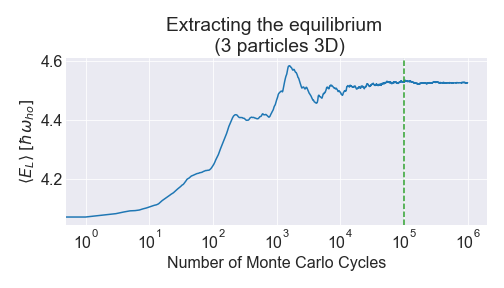
\includegraphics[width=0.7\linewidth]{../Results/equilibrium}\caption{The relationship between the number of MC cycles and the expectation value. The dotted line represents the choice of equilibration.}\label{fig:equilibrium}
\end{figure} 


\newpage
%\begin{multicols}{2}\footnotesize
\bibliographystyle{unsrt}%unsrt
\bibliography{References}
%\end{multicols}
\end{document}